\chapter{Future Work}

In this section, we discuss the use of neural Bayesian learning to synthesize
control of robotic systems with contact. 

\section{Bayesian Policy Learning with Contact}

Contact-rich dynamical systems~\cite{bhounsule2016dead,
sirichotiyakul2019energetically, ashenafi2021nonholonomic}, such as walking
robots and multi-fingered grippers, require complex control design techniques.
In recent years, policies generated from data-driven techniques have shown the
potential to balance contact forces, break and reestablish contact while
maintaining control of the overall system~\cite{nagabandi2020deep}. Inspired by
these techniques, we leverage the robustness properties of data-driven NBL to
design controllers for robotic manipulation and locomotion with contact.
Moreover, we will utilize NBL to infer a stochastic controller that can account
for uncertainties in the hybrid dynamical system, such as friction and
unmodelled dynamics. This can be achieved by designing a controller for a wide
range of uncertain system parameters such that a single controller performs well
for various environmental conditions.

The NBL optimization problem given in~\eqref{eq:neural_bayesian_inference}
requires knowledge of the system model and tools to take gradient through the
differential equations governing the dynamics of the system. In recent years,
advancements in system modeling and control have allowed for modeling contacts
accurately and take gradients through these contact models. A brief summary of
these techniques are discussed as follows:

\begin{enumerate}
    \item Linear Complementarity Problem (LCP) : the LCP formulation presented
    in~\cite{glocker2005formulation} provides a convex optimization problem that
    resolves contacts, impacts and Coulomb friction. This formulation combats
    paradoxes exhibited by other contact modeling techniques, such as event
    detection and compliance contact models.
    \item Gradients through a convex optimization : formulations given
    in~\cite{de2018end} and~\cite{amos2019differentiable} provide a technique to
    take gradients through a convex optimization problem. This allows us to
    compute jacobian of linear complementarity problems in order to learn a
    viable control law through NBL.
\end{enumerate}

The objectives of the proposed research plan can be summarized as follows.
\begin{enumerate}
    \item Learn deterministic policies for dynamical systems with contacts by
    solving the following optimization problem.
    \begin{equation}
        \begin{aligned}
            \underset{\theta }{\textrm{minimize}} 
            &&\quad J(&\phi(t; x_0, u), u) \\
            \textrm{subject to} 
            &&\quad M(x)\dd x &- h(x, \dot{x}, u) \dd t - \dd \Lambda= 0, \\
            &&\quad u(x; \theta) &= g \circ F(x; \theta),
        \end{aligned}    
        \label{eq:deter_lcp_opt}%
      \end{equation}
    where $M$ is the mass matrix, $h$ holds Coriolis terms and generalized
    forces and $\Lambda$ holds the normal and tangential contact forces on the
    system~\cite{glocker2005formulation}.
    \item Learn stochastic policies for contact-rich systems that work under
    various environmental conditions with uncertain characteristics, such as
    friction, represented by the parameters $\mu$. The resulting NBL
    optimization problem can be written as
      \begin{equation}
        \begin{aligned}
            \underset{q(\theta) }{\textrm{minimize}} 
            &&\quad J(&\phi(t; x_0, u), u) \\
            \textrm{subject to} 
            &&\quad M(x)\dd x &- h(x, \dot{x}, u) \dd t - \dd \Lambda(\mu)= 0, \\
            &&\quad u(x; \theta) &= g \circ F(x; \theta), \\
            &&\quad \mu &\sim \mathcal{N}(\mu_0, \sigma_\mu), \\
            &&\quad \theta &\sim q(\theta).
        \end{aligned}    
        \label{eq:bays_lcp_opt}%
      \end{equation}
\end{enumerate}


We will test the performance of the deterministic and stochastic policies on the
rimless-wheel system~\cite{sirichotiyakul2019energetically}. As shown in
Figure~\ref{fig:rimless}, the system pivots on one spoke at a time to mimic the
gait of an underactuated walking robot. The wheel is actuated by a pendulum
attached at the base of the spokes. The objective is to learn a robust and 
stable controller that drives the system to a desirable limit cycle.
% \subsection{Learning the Form of the Model}

\begin{figure}[H]
    \centering
    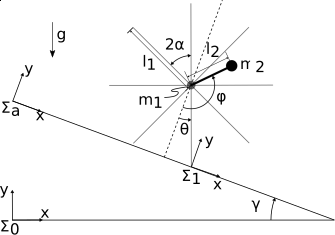
\includegraphics[width=0.4\linewidth]{./figures/rimless_wheel.jpg}
    \caption{Pendulum-driven rimless wheel~\cite{bhounsule2016dead}}
    \label{fig:rimless}
\end{figure}
\section{Schedule}

\begin{table}[H]
    \centering
    \caption{Schedule}
    % \rowcolors{2}{}{Wheat1}
    \begin{tabular}{|c|c|}
    \toprule
    %   & \multicolumn{2}{c}{Framework} \\
    %   \cmidrule(lr){2-3}
    \textbf{Timeline} & \textbf{Task} \\
    \midrule 
    \midrule
        August - September 2022 & Learn deterministic policy of the rimless-wheel \\ 
        October - November 2022 & Learn stochastic policy of the rimless-wheel \\
        November - December 2022 & Submit work to a journal publication \\
        December 2022 - February 2023 & Write dissertation \\
        March - May 2023 & Prepare dissertation presentation and defend \\
    \bottomrule
    \end{tabular}
    \label{tab:training_setup_neuralpbc}
\end{table}

